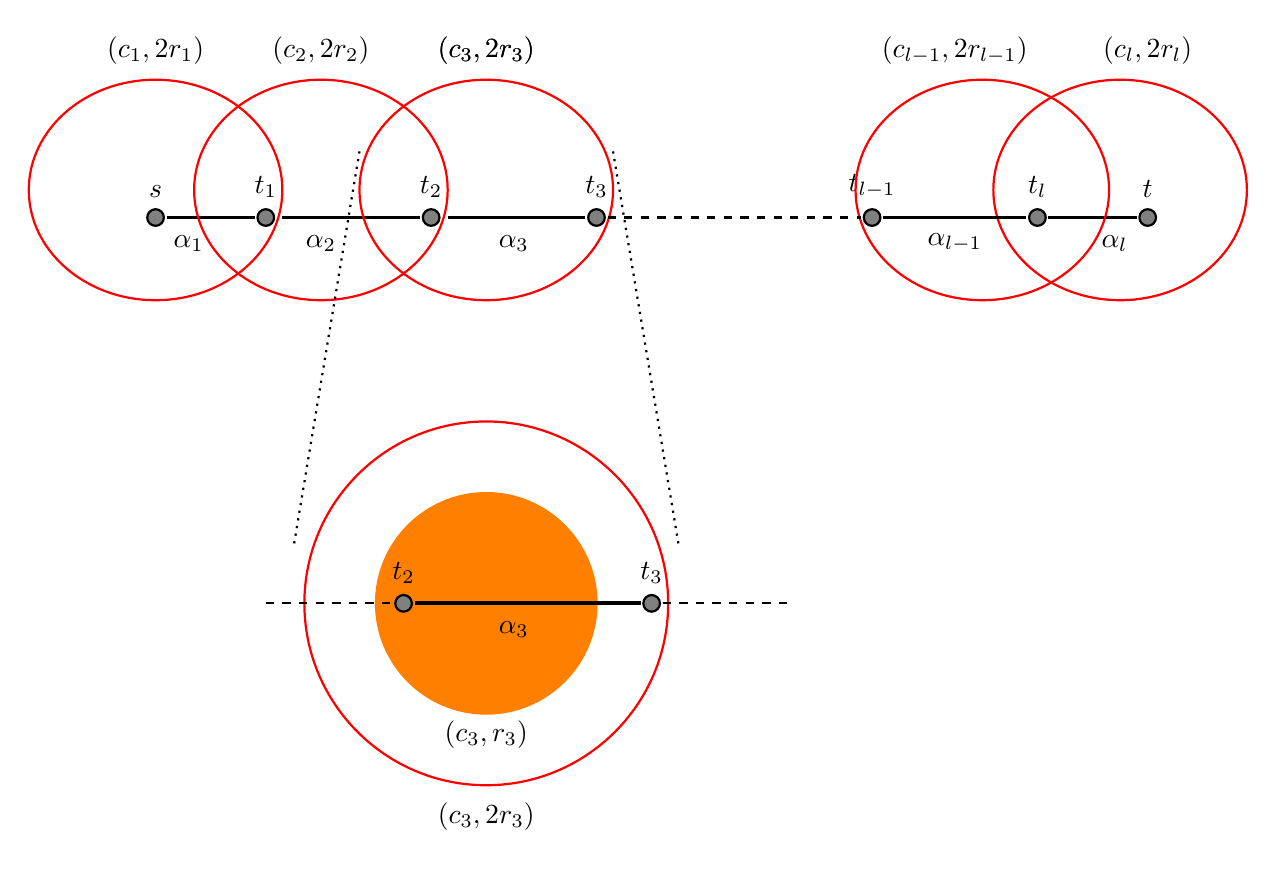
\begin{tikzpicture}[thick,scale=0.7]
	\draw (0, 0) node[circle, draw, fill=black!50, inner sep=0pt, minimum width=6pt, label = $s$] {};
	\draw (18, 0) node[circle, draw, fill=black!50, inner sep=0pt, minimum width=6pt,label = $t$] {};
	
	\draw (2, 0) node[circle, draw, fill=black!50, inner sep=0pt, minimum width=6pt,label = $t_1$] {};
	\draw [line width = 0.5mm] (0.2, 0) -- (1.8, 0);
	\draw (0.6, -1) node[red, label={$\alpha_1$}]{};
	\draw [red] (0, 0.5) ellipse (2.3 and 2);
	\draw (0, 2.4) node[red, label={$\ball(c_1, 2r_{1})$}]{};
	
	\draw (5, 0) node[circle, draw, fill=black!50, inner sep=0pt, minimum width=6pt,label = $t_2$] {};
	\draw [line width = 0.5mm] (2.3, 0) -- (4.8, 0);
	\draw (3, -1) node[red, label={$\alpha_2$}]{};
	\draw [red] (3, 0.5) ellipse (2.3 and 2);
	\draw (3, 2.4) node[red, label={$\ball(c_2, 2r_{2})$}]{};
	
	\draw (8, 0) node[circle, draw, fill=black!50, inner sep=0pt, minimum width=6pt,label = $t_3$] {};
	\draw [line width = 0.5mm] (5.3, 0) -- (7.8, 0);
	\draw (6.5, -1) node[red, label={$\alpha_3$}]{};
	\draw [red] (6, 0.5) ellipse (2.3 and 2);
	\draw (6, 2.4) node[red, label={$\ball(c_3, 2r_{3})$}]{};
	
	\draw[dotted] (3.7, 1.2) -- (2.5, -6);
	\draw[dotted] (8.3, 1.2) -- (9.5, -6);
	\draw [fill=orange,orange] (6, -7) ellipse (2 and 2);
	\draw (6, -10) node[red, label={$\ball(c_3, r_{3})$}]{};
	\draw (4.5, -7) node[circle, draw, fill=black!50, inner sep=0pt, minimum width=6pt,label = $t_2$] {};
	\draw (9, -7) node[circle, draw, fill=black!50, inner sep=0pt, minimum width=6pt,label = $t_3$] {};
	\draw [red] (6, -7) ellipse (3.3 and 3.3);
	\draw (6, -11.5) node[red, label={$\ball(c_3, 2r_{3})$}]{};
	\draw (6, 2.4) node[red, label={$\ball(c_3, 2r_{3})$}]{};
	\draw [line width = 0.5mm] (4.7, -7) -- (8.8, -7);
	\draw (6.5, -8) node[red, label={$\alpha_3$}]{};
	\draw [dashed] (2, -7) -- (4.3, -7);
	\draw [dashed] (9.2, -7) -- (11.5, -7);
	
	
	\draw (16, 0) node[circle, draw, fill=black!50, inner sep=0pt, minimum width=6pt,label = $t_l$] {};
	\draw [line width = 0.5mm] (17.8, 0) -- (16.2, 0);
	\draw (17.4, -1) node[red, label={$\alpha_l$}]{};
	\draw [red] (17.5, 0.5) ellipse (2.3 and 2);
	\draw (18, 2.4) node[red, label={$\ball(c_l, 2r_{l})$}]{};
	
	\draw (13, 0) node[circle, draw, fill=black!50, inner sep=0pt, minimum width=6pt,label = $t_{l-1}$] {};
	\draw [line width = 0.5mm] (15.8, 0) -- (13.2, 0);
	\draw (14.5, -1) node[red, label={$\alpha_{l-1}$}]{};
	\draw [red] (15, 0.5) ellipse (2.3 and 2);
	\draw (14.5, 2.4) node[red, label={$\ball(c_{l-1}, 2r_{l-1})$}]{};
	
	\draw [dashed] (8.2, 0) -- (12.8, 0); 
\end{tikzpicture}